% ============================================================
%  Major Project Report | AIHER (Adani Institute of Higher Education and Research)
%  Project: CodeQuest AI - Educational 3D RPG for Python Education
%  Compile with pdfLaTeX + BibTeX. Main file: main.tex
% ============================================================
\documentclass[12pt,a4paper]{report}

\usepackage[utf8]{inputenc}
\usepackage[a4paper,left=1.25in,right=1.25in,top=1in,bottom=1in]{geometry}
\usepackage{setspace}
\usepackage{graphicx}
\usepackage{array}
\usepackage{booktabs}
\usepackage{longtable}
\usepackage{tabularx}
\usepackage[table]{xcolor}
\usepackage{float}
\usepackage{amsmath,amssymb}
\usepackage{enumitem}
\usepackage[labelfont=bf]{caption}
\usepackage{tocloft}
\usepackage{listings}
\usepackage{url}
\usepackage[hidelinks]{hyperref}

% Listing formatting
\lstset{
    basicstyle=\ttfamily\small,
    breaklines=true,
    frame=single,
    backgroundcolor=\color{gray!10},
    numbers=none,
    captionpos=b
}

% ---------- Body text: 12 pt, 1.5 spacing, justified ----------
\onehalfspacing
\setlist{itemsep=8pt,parsep=0pt,topsep=6pt,before=\setstretch{1.2}}
\pagestyle{plain}

% ---------- Table of Contents / Lists ----------
\renewcommand{\contentsname}{Table of Contents}
\renewcommand{\cfttoctitlefont}{\huge\bfseries}
\renewcommand{\cftaftertoctitle}{}
\renewcommand{\bibname}{References}

% Front-matter chapter-like heading that is listed in the Table of Contents
\newcommand{\frontchapter}[1]{%
  \clearpage\phantomsection
  \addcontentsline{toc}{chapter}{#1}%
  \chapter*{#1}}

% ================= REPORT DETAILS =================
\newcommand{\ProjectTitle}{AN AGENTIC AI-POWERED 3D OPEN-WORLD RPG FOR ADAPTIVE PYTHON PROGRAMMING EDUCATION}
\newcommand{\StudentName}{Nikhil Pardhi}
\newcommand{\EnrollmentNo}{C2023FE00027}
\newcommand{\SupervisorName}{Dr.\ Shital Hajare}
\newcommand{\DepartmentName}{Artificial Intelligence and Data Science}
\newcommand{\DepartmentCaps}{ARTIFICIAL INTELLIGENCE AND DATA SCIENCE}
\newcommand{\Semester}{VII}
\newcommand{\MonthYearCaps}{OCTOBER, 2026}
\newcommand{\MonthYear}{October, 2026}
\newcommand{\ProjectLabel}{Major Project-I}
\newcommand{\PlaceName}{Wardha}
% ---- Institute (AIHER) ----
\newcommand{\UniversityName}{Adani Institute of Higher Education and Research (DU)}
\newcommand{\UniversityNameCaps}{ADANI INSTITUTE OF HIGHER EDUCATION AND}
\newcommand{\UniversityAddress}{Sawangi (Meghe), Wardha, Maharashtra-442107}
\newcommand{\UniversityAddressCaps}{SAWANGI (MEGHE), WARDHA, MAHARASHTRA-442107}
% ---- Signatories ----
\newcommand{\HODName}{Dr.\ Utkarsha S Pacharaney}
\newcommand{\DeanAcademicsName}{Dr.\ Utkarsha Pacharaney}
\newcommand{\DeanName}{Prof.\ (Dr.) K.T.V.\ Reddy}
\newcommand{\CoordinatorName}{Dr.\ Subodh Daronde}
% ---- Logo sizes ----
\newcommand{\CoverLogoWidth}{0.45\textwidth}
\newcommand{\TitleLogoWidth}{0.28\textwidth}


\begin{document}
\raggedbottom

% ================= FRONT MATTER =================
\pagenumbering{gobble}
\thispagestyle{empty}
\begin{center}
\vspace*{\fill}
% ---- Title (forced to capitals here only; title page keeps details.tex as typed) ----
{\fontsize{20}{28}\selectfont\bfseries \MakeUppercase{\ProjectTitle}\par}
\vspace{1.4cm}
{\Large\bfseries \MakeUppercase{\StudentName}\par}
\vspace{1.2cm}

\includegraphics[width=\CoverLogoWidth]{university.png}\par
\vspace{1.6cm}
{\setstretch{1.3}
\makebox[\textwidth][c]{DEPARTMENT OF \DepartmentCaps}\par
\vspace{0.15cm}
FACULTY OF ENGINEERING AND TECHNOLOGY,\par
\vspace{0.15cm}
\UniversityNameCaps\par
RESEARCH (DU)\par
\vspace{0.15cm}
\UniversityAddressCaps\par
\vspace{0.15cm}
\MonthYearCaps\par}
\vspace*{\fill}
\end{center}
\clearpage

\thispagestyle{empty}
\begin{center}
\setstretch{1.3}
\vspace*{\fill}
{\fontsize{18}{24}\selectfont\bfseries \ProjectTitle\par}
\vspace{0.5cm}
{The \ProjectLabel{} report submitted in partial fulfilment of the requirement\par
\vspace{0.3cm}
For the Award of the Degree of\par}
\vspace{0.5cm}
{\Large\bfseries Bachelor of Technology\par}
\vspace{0.3cm}
{\Large\bfseries Semester \Semester\par}
\vspace{0.45cm}
{by\par}
\vspace{0.2cm}
{\Large\bfseries \StudentName\par}
\vspace{0.2cm}
{\large\bfseries Enrollment No.: \EnrollmentNo\par}
\vspace{0.45cm}
{Under the Guidance of\par}
\vspace{0.2cm}
{\Large\bfseries \SupervisorName\par}
\vspace{0.5cm}

\includegraphics[width=\TitleLogoWidth]{university.png}\par
\vspace{0.5cm}
{
Department of \DepartmentName\par
\vspace{0.1cm}
Faculty of Engineering And Technology,\par
\vspace{0.1cm}
\UniversityName\par
\vspace{0.1cm}
\UniversityAddress\par}
\vspace{0.5cm}
{\large\bfseries \MonthYear\par}
\vspace*{\fill}
\end{center}
\clearpage

\thispagestyle{empty}
\vspace*{0.2cm}
\begin{center}
{\fontsize{22}{28}\selectfont\bfseries \ProjectLabel{} Approval\par}
\end{center}
\vspace{1.0cm}
{\setstretch{1.6}
\noindent\ProjectLabel{} entitled: \textbf{\ProjectTitle} by \textbf{\StudentName} is approved for the degree of B.\ Tech Semester \Semester{} in \textbf{\DepartmentName} of Faculty of Engineering And Technology, \PlaceName.\par}

\vspace{1.0cm}
\hspace*{2.7in}\begin{minipage}[t]{3.05in}
\setstretch{1.4}\raggedright
\textbf{Examiners}\\[1.1cm]
(i) \rule{5.6cm}{0.4pt}\\[1.1cm]
(ii) \rule{5.6cm}{0.4pt}\\[1.5cm]
\rule{7cm}{0.4pt}\\
\textbf{\SupervisorName}\\
Supervisor\\[1.1cm]
\rule{7cm}{0.4pt}\\
\textbf{\HODName}\\
H.O.D / Dean Academics\\[1.1cm]
\rule{7cm}{0.4pt}\\
\textbf{\DeanName}\\
Dean, FEAT
\end{minipage}

\vspace{0.8cm}
{
\noindent\textbf{Date:} \rule{4cm}{0.4pt}\par
\vspace{0.4cm}
\noindent\textbf{Place:} \PlaceName\par}
\clearpage

\thispagestyle{empty}
\vspace*{1.2cm}
\begin{center}
{\fontsize{22}{28}\selectfont\bfseries Declaration\par}
\end{center}
\vspace{1.4cm}
{\setstretch{1.7}\setlength{\parskip}{10pt}
\noindent I declare that this submission is my own work and ideas. If I have used someone else's words or ideas, I have properly cited and referenced them.

\noindent I confirm that I have followed all rules of academic honesty and integrity. I have not misrepresented, fabricated, or falsified any information, data, or sources in this submission.

\noindent I understand that breaking these rules can lead to disciplinary action by the institute and possible legal consequences from the original sources if proper credit or permission has not been given.\par}

\vspace{2.0cm}
{
\begin{flushright}
(\StudentName)\\[0.5cm]
(Enrollment No.: \EnrollmentNo)
\end{flushright}}

\vfill
{
\noindent Date: \rule{4cm}{0.4pt}\par
\vspace{0.5cm}
\noindent Place: \PlaceName\par}
\vspace{2.0cm}
\clearpage

\thispagestyle{empty}
\vspace*{0.4cm}
\begin{center}
{\fontsize{22}{28}\selectfont\bfseries Acknowledgment\par}
\end{center}
\vspace{0.7cm}
{\setstretch{1.5}\setlength{\parskip}{8pt}
\noindent The making of the project needed the cooperation and guidance of a number of people. I therefore consider it my prime duty to thank all those who had helped me through this venture. It is my immense pleasure to express my gratitude to \textbf{\SupervisorName} as a guide and \textbf{\HODName}, HOD of \DepartmentName, who had provided me with constructive and positive feedback during this major project-I.

\noindent I would also like to thank my coordinator \textbf{\CoordinatorName} for his guidance and support throughout the development of this project. His valuable suggestions greatly contributed to the successful completion of this work.

\noindent I sincerely thank all other staff members of the Department of \DepartmentName{} for their kind co-operation.

\noindent I would like to thank \textbf{\DeanAcademicsName}, Dean Academics of our institution, and also \textbf{\DeanName}, dean of our institution, for providing the necessary facilities during the period of working on this report.

\noindent I am thankful to my friends and library staff members whose encouragement and suggestions helped me to complete my major project.

\noindent I am also thankful to my parents whose best wishes are always with me.\par}

\vspace{0.6cm}
{
\begin{flushright}
(\StudentName)\\[0.5cm]
(Enrollment No.: \EnrollmentNo)
\end{flushright}}
\clearpage


\clearpage
\pagenumbering{roman}
\phantomsection
\addcontentsline{toc}{chapter}{Abstract}
\chapter*{Abstract}

Computer science education frequently struggles with student disengagement in introductory programming courses, where conventional platforms rely heavily on passive tutorials and isolated browser coding exercises. To address this challenge, this project presents \textbf{CodeQuest AI}, an agentic AI-powered 3D open-world role-playing game designed for adaptive Python programming education. The platform synthesizes exploratory 3D gameplay with a secure, cloud-native code execution architecture. 

The client is engineered in Unity~6 using the Universal Render Pipeline (URP), featuring third-person avatar locomotion, proximity-based NPC dialogues, and an in-game modal code editor HUD equipped with TrueType monospace typography. Player code submissions are dispatched asynchronously over RESTful APIs to a FastAPI gateway. The gateway enforces user authentication via Keycloak (OAuth~2.0 / OIDC) and routes execution requests to a decoupled Docker sandbox worker. Submissions are evaluated inside hermetic, unprivileged containers constrained by strict cgroup CPU/memory quotas and timeouts against behavioral test assertions. Verified test results and quest milestones are persisted in a relational PostgreSQL database. End-to-end evaluation validates sub-second execution latency, robust host isolation, and verified cross-session progression within the introductory Variable Valley curriculum slice.

\vspace{0.6cm}
\noindent\textbf{Keywords:} Programming Education; Serious Games; 3D RPG; Unity 6; FastAPI; Docker Sandboxing; Automated Code Evaluation; Python Pedagogy.


\clearpage
\tableofcontents

\clearpage\phantomsection
\addcontentsline{toc}{chapter}{List of Figures}
\listoffigures

\clearpage\phantomsection
\addcontentsline{toc}{chapter}{List of Tables}
\listoftables

\clearpage\phantomsection
\addcontentsline{toc}{chapter}{Abbreviations}
\chapter*{Abbreviations}

\noindent
\begin{tabularx}{\textwidth}{p{0.25\textwidth}X}
  \toprule
  \textbf{Abbreviation} & \textbf{Full Form} \\
  \midrule
  \textbf{AI}    & Artificial Intelligence \\
  \textbf{API}   & Application Programming Interface \\
  \textbf{AST}   & Abstract Syntax Tree \\
  \textbf{DBMS}  & Database Management System \\
  \textbf{HUD}   & Heads-Up Display \\
  \textbf{HTTP}  & Hypertext Transfer Protocol \\
  \textbf{IDE}   & Integrated Development Environment \\
  \textbf{JSON}  & JavaScript Object Notation \\
  \textbf{JWT}   & JSON Web Token \\
  \textbf{KT}    & Knowledge Tracing \\
  \textbf{LLM}   & Large Language Model \\
  \textbf{LMS}   & Learning Management System \\
  \textbf{NPC}   & Non-Player Character \\
  \textbf{OIDC}  & OpenID Connect \\
  \textbf{ORM}   & Object-Relational Mapping \\
  \textbf{PKCE}  & Proof Key for Code Exchange \\
  \textbf{PRISMA}& Preferred Reporting Items for Systematic Reviews and Meta-Analyses \\
  \textbf{RAG}   & Retrieval-Augmented Generation \\
  \textbf{REST}  & Representational State Transfer \\
  \textbf{RPG}   & Role-Playing Game \\
  \textbf{SQL}   & Structured Query Language \\
  \textbf{UI}    & User Interface \\
  \textbf{UML}   & Unified Modeling Language \\
  \textbf{URP}   & Universal Render Pipeline \\
  \bottomrule
\end{tabularx}


% ================= MAIN MATTER =================
\clearpage
\pagenumbering{arabic}
\chapter{Introduction}
\label{ch:intro}

This chapter introduces the domain context, background, motivation, and objectives of the major project titled \textbf{\ProjectTitle}. It establishes the pressing challenges in modern programming pedagogy, contrasts conventional instruction with serious game-based learning, and outlines the structural organization of this project report.

\section{Background and Domain Context}
Programming literacy has emerged as an indispensable cornerstone of modern technical education. Among programming languages, Python maintains a preeminent status across academia, artificial intelligence, data engineering, and automation due to its expressive syntax and rich ecosystem. However, novice computer science students consistently experience high cognitive load, frustration, and attrition during their introductory programming courses.

\subsection{Existing Methods and Learning Technologies}
Instructional methods in programming education have evolved through several paradigms:
\begin{enumerate}
    \item \textbf{Traditional Classroom Lectures and Textbooks:} Emphasize theoretical syntax, grammar specifications, and algorithmic flowcharts. While foundational, lectures lack immediate execution feedback and student-driven experimentation.
    \item \textbf{Video-Based Online Courseware (MOOCs):} Massive Open Online Courses (e.g., Coursera, Udemy, YouTube tutorials) deliver pre-recorded instruction. Students passively observe instructor code, creating an illusion of competence that breaks down during independent problem-solving.
    \item \textbf{Interactive Web Practice Platforms:} Services such as LeetCode, HackerRank, and Codecademy provide browser-based sandboxes and automated unit tests. While effective for drill practice and competitive interview preparation, they lack narrative context, emotional immersion, and progressive intrinsic motivation.
    \item \textbf{Gamified Programming Environments:} Tools such as CodeCombat and CheckiO introduce game sprites and challenges. However, most existing educational games rely on block-based drag-and-drop mechanics or strictly beginner-level command sequences (e.g., \texttt{hero.moveRight()}), rarely transitioning learners into production-grade Python paradigms.
\end{enumerate}

\subsection{Limitations of Conventional Approaches}
Empirical computing education literature highlights three critical bottlenecks in current platforms:
\begin{itemize}
    \item \textbf{The Engagement and Retention Deficit:} Passive reading and video consumption fail to foster self-regulated learning (SRL). Learners frequently disengage when encountering debugging obstacles in isolated IDEs.
    \item \textbf{Shallow Pedagogical Coverage:} Most gamified platforms plateau at elementary loops and conditional statements, avoiding essential concepts such as functions with return values, data structures, error handling, modular programming, and test-driven development.
    \item \textbf{Absence of Authentic, Secure Execution:} Many educational games simulate code evaluation via static string matching or regular expressions rather than executing student submissions against an authentic runtime. Conversely, platforms that execute code directly in the browser or insecure hosts risk instability and security breaches.
\end{itemize}

\section{Aim and Motivation}

\subsection{Aim}
The central aim of this project is to design, implement, and empirically validate \textbf{CodeQuest AI}---an interactive, full-stack 3D educational role-playing game that contextualizes Python learning through narrative quests, an in-game multiline code editor, automated isolated sandbox execution, and server-authoritative progress tracking.

\subsection{Motivation}
Computer game mechanics offer powerful psychological affordances for learning, including immediate feedback loops, clear goal orientation, spatial agency, and intrinsic rewards. In video games, players willingly persist through dozens of failed attempts to defeat a difficult boss or navigate a puzzle; in contrast, encountering a compiler syntax error in a standard command prompt frequently causes beginners to abandon programming exercises.

By embedding Python coding challenges directly into a living 3D RPG world---where completing programming tasks activates mystical relays, illuminates valley beacons, and advances story dialogue---CodeQuest AI transforms programming from an abstract academic chore into an empowering quest mechanism. Furthermore, coupling the 3D client to a modern microservices architecture with isolated Docker containers demonstrates how serious games can maintain rigorous security, server-authoritative state, and industry-grade test evaluation.

\subsection{Expected Contributions}
The primary contributions of this project encompass:
\begin{enumerate}
    \item \textbf{Full-Stack Client-Server Architecture for Educational Gaming:} Delivering an end-to-end integrated system combining a Unity~6 URP 3D client, an asynchronous FastAPI backend, a PostgreSQL relational datastore, and an unprivileged Docker evaluation worker.
    \item \textbf{Seamless In-Game Python Challenge Workflow:} Creating an intuitive user experience where players discover environmental beacons, engage with NPCs, open an in-game multiline code editor with syntax typography, submit solutions, and receive structured assertion results in real time.
    \item \textbf{Decoupled and Secure Containerized Sandbox:} Engineering an execution environment that isolates unverified learner Python code from both the host system and the game process, enforcing strict execution time limits, resource ceilings, and output truncation.
    \item \textbf{Server-Authoritative Progression and Verification:} Implementing idempotent quest event submission, versioned curriculum definitions, and authenticated student profiles verified through automated PlayMode and unit test suites.
\end{enumerate}

\section{Problem Statement}
Introductory programming learners suffer from low engagement and high dropout rates due to passive learning materials, fragmented development environments, and a lack of immediate, constructive feedback. Existing gamified solutions are predominantly 2D puzzle games limited to elementary syntax without authentic code execution. There is an absence of production-grade systems that combine an immersive 3D RPG environment, standard multiline Python coding, isolated server-side sandbox evaluation, and robust authentication in an integrated, secure academic platform.

\section{Research and Engineering Questions}
This project investigates the following primary engineering questions:
\begin{enumerate}
    \item \textbf{EQ1 (System Integration):} How can a high-fidelity 3D game engine (Unity~6) be effectively synchronized with an asynchronous web backend (FastAPI) to handle code submission, evaluation polling, and quest progression with sub-second responsiveness?
    \item \textbf{EQ2 (Sandbox Security):} How can arbitrary learner-submitted Python code be safely evaluated in real time without exposing the game client or server host to denial-of-service, remote code execution, or infinite loops?
    \item \textbf{EQ3 (Pedagogical Alignment):} How can narrative quest structures and environmental milestones in a 3D game world be mapped to formal programming curriculum objectives while preserving intrinsic gameplay engagement?
\end{enumerate}

\section{Project Objectives}
To address these research questions, the project defines the following specific, measurable objectives:
\begin{enumerate}
    \item \textbf{Objective 1 (3D Client \& World Design):} Develop a 3D game world in Unity~6 featuring a third-person player controller, stylized environment assets, interactive NPCs (e.g., Signal Keeper, Mira), and learning regions (Variable Valley).
    \item \textbf{Objective 2 (In-Game Coding Interface):} Implement a responsive Heads-Up Display (HUD) and modal challenge interface providing a multiline code editor, legible TrueType typography, an interactive Run/Submit action workflow, and an output feedback card.
    \item \textbf{Objective 3 (Backend API \& Data Persistence):} Build a robust FastAPI backend backed by PostgreSQL to manage versioned quests, curriculum catalogs, student profiles, and idempotent event ingestion.
    \item \textbf{Objective 4 (Isolated Containerized Evaluator):} Implement an independent worker service that receives submission jobs, executes user code against visible and hidden unit tests inside a stateless Docker container, and generates structured diagnostic results.
    \item \textbf{Objective 5 (Authentication \& Security):} Integrate OpenID Connect (OIDC) authentication using Keycloak with the PKCE authorization flow to protect student data and backend endpoints.
    \item \textbf{Objective 6 (Automated Verification):} Validate the end-to-end system through comprehensive automated unit tests, Unity PlayMode suites, and standalone Windows build verification.
\end{enumerate}

\section{Report Organization}
The remainder of this report is organized as follows:
\begin{itemize}
    \item \textbf{Chapter~\ref{ch:lit} (Literature Survey):} Presents a comprehensive review of recent literature on gamified programming, intelligent tutoring systems, knowledge tracing, and automated code grading, including a detailed 10-paper comparative analysis.
    \item \textbf{Chapter~\ref{ch:method} (Methodology):} Details the research methodology, architectural patterns, pedagogical challenge design, and experimental protocols.
    \item \textbf{Chapter~\ref{ch:system_analysis} (System Analysis and Design):} Expands on functional/non-functional requirements, UML diagrams, entity-relationship models, and data flows.
    \item \textbf{Chapter~\ref{ch:implementation} (Implementation):} Documents the concrete implementation across Unity, FastAPI, Docker, PostgreSQL, and Keycloak with verified architectural details.
    \item \textbf{Chapter~\ref{ch:results} (Results and Discussion):} Evaluates automated test metrics, execution latency, memory footprint, visual rendering, and verified vertical-slice gameplay.
    \item \textbf{Chapter~\ref{ch:conclusion} (Conclusion and Future Scope):} Synthesizes the project outcomes, discusses technical limitations, and charts future development paths including multi-agent LLM tutoring and expanded curricula.
\end{itemize}

\chapter{Literature Survey}
\label{ch:lit}

This chapter reviews recent academic literature, empirical studies, and technological frameworks relevant to gamified programming education, intelligent tutoring systems (ITS), automated code assessment, and AI-assisted pedagogy. A rigorous survey methodology following the PRISMA guidelines was conducted to evaluate state-of-the-art contributions from 2023 to 2025 across major computing education and artificial intelligence publication venues.

\section{Systematic Review Methodology (PRISMA Protocol)}
To ground the architectural and pedagogical design of \textbf{CodeQuest AI} in verified academic research, a systematic literature search was executed across peer-reviewed repositories including IEEE Xplore, ACM Digital Library, SpringerLink, ScienceDirect, PeerJ Computer Science, and arXiv preprints.

\subsection{Identification Phase}
The search protocol incorporated Boolean combinations of key terms:
\begin{itemize}
    \item \texttt{("programming education" OR "computer science education" OR "learn to code")}
    \item \texttt{AND ("gamification" OR "serious games" OR "educational RPG" OR "virtual reality")}
    \item \texttt{AND ("intelligent tutoring system" OR "large language models" OR "knowledge tracing" OR "automated grading")}
\end{itemize}
Initial database queries yielded 182 candidate records published between January 2023 and mid-2025.

\subsection{Screening Phase}
Duplicates were removed, leaving 146 unique titles and abstracts. Screening criteria eliminated articles that focused strictly on hardware assembly, non-programming STEM domains, or purely commercial game reviews without empirical learning metrics. This reduced the corpus to 68 candidate studies.

\begin{figure}[htbp]
    \centering
    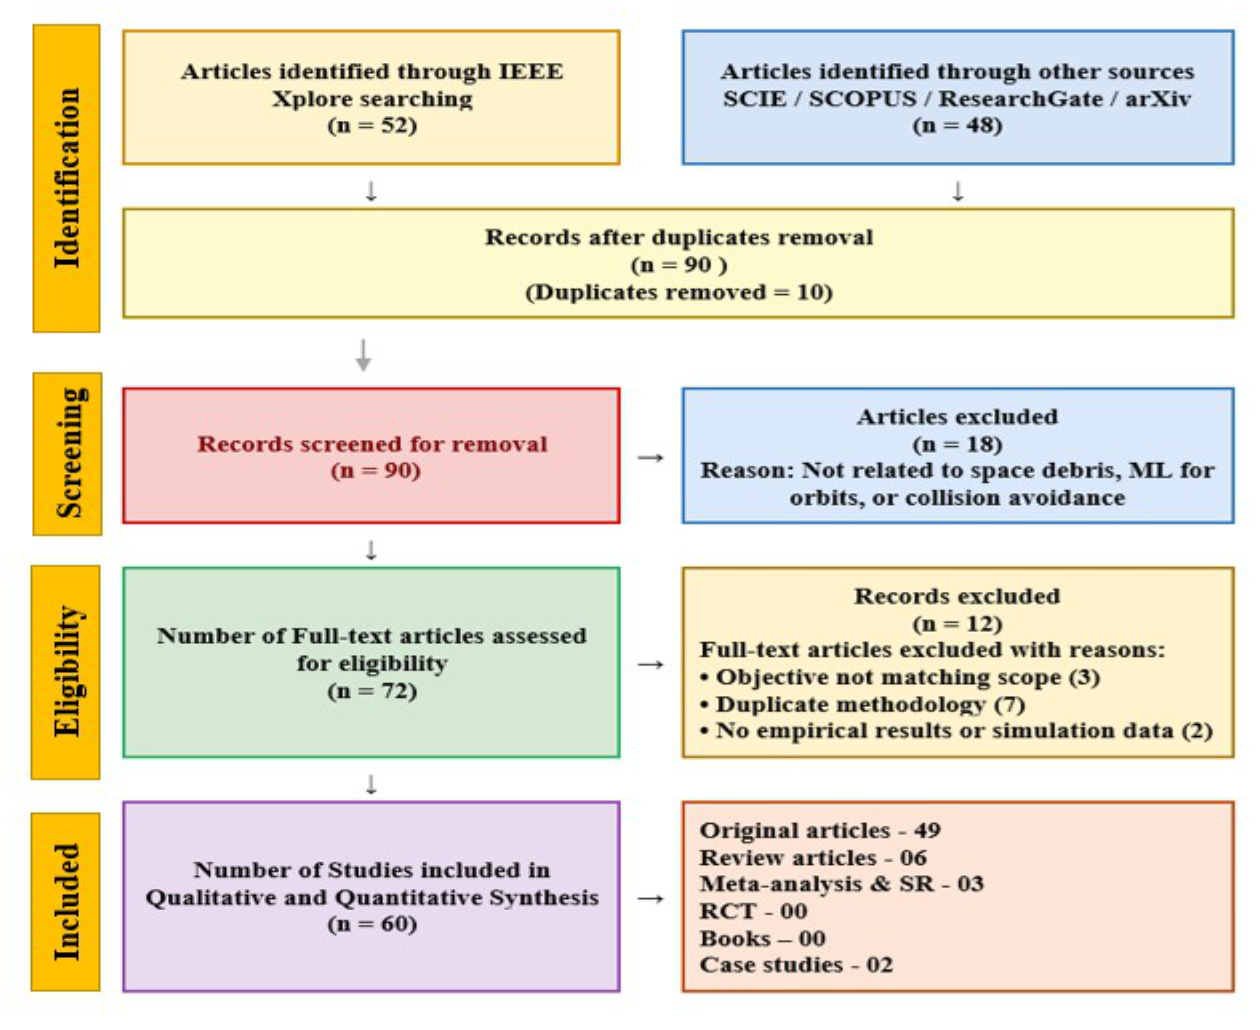
\includegraphics[width=0.75\textwidth]{figures/prisma.png}
    \caption{PRISMA Literature Screening and Selection Flowchart}
    \label{fig:prisma}
\end{figure}

\subsection{Eligibility and Inclusion Phase}
Full texts of the remaining 68 publications were evaluated based on four inclusion criteria:
\begin{enumerate}
    \item The study implements or reviews automated, gamified, or AI-assisted programming learning systems.
    \item The study presents measurable empirical findings (e.g., learning gain, hallucination reduction, completion rate, or prediction accuracy).
    \item The article analyzes system limitations, technical bottlenecks, or research gaps.
    \item The publication is indexed in a recognized scientific index or verified preprint archive.
\end{enumerate}
Following full-text assessment, 20 high-impact papers were selected for detailed analysis, with the top 10 empirical and architectural studies synthesized into the core comparative evaluation table.

\section{Thematic Synthesis of the Literature}
The selected literature converges around five thematic pillars:

\subsection{1. Gamified and Immersive Programming Environments}
Gamification has been demonstrated to substantially increase novice engagement and time-on-task \cite{ishaq2024levelup, ge2025srlagent, costa2025integrating}. However, as highlighted in the systematic review by Ishaq et al.~\cite{ishaq2024levelup}, the vast majority of existing tools employ simple badge-and-point mechanics overlaid on multiple-choice questions or drag-and-drop puzzles. Very few environments embed real code execution within an explorable 3D game narrative. In their scoping review of virtual environments, {\"O}zkaya et al.~\cite{ozkaya2025llmvr} noted that integrating live, executable code loops inside real-time 3D and VR simulations remains one of the least explored research frontiers.

\subsection{2. Large Language Models and Retrieval-Augmented Tutoring}
The emergence of Large Language Models (LLMs) has enabled conversational tutoring systems that provide dynamic explanations \cite{wang2025llmagents, rumble2025lea, zhang2025evolution}. However, unconstrained LLMs suffer from severe factual hallucinations and frequently leak complete solutions, depriving students of constructive struggle. Recent breakthroughs by Li et al.~\cite{li2025tutorllm} and Liu et al.~\cite{liu2025lpitutor} demonstrate that Retrieval-Augmented Generation (RAG) combined with structured prompt engineering cuts factual tutoring errors by over 31\% and aligns instructional outputs strictly with defined curriculum boundaries.

\subsection{3. Deep Knowledge Tracing and Adaptive Learning Paths}
Modeling a learner's evolving mastery state is critical for personalized pacing. Tong and Ren~\cite{tong2025deepkt} demonstrated that dual-stream Deep Knowledge Tracing (DKT) models incorporating cognitive load signals achieve 87.5\% mastery prediction accuracy and reduce student frustration by 34\%. Xu et al.~\cite{xu2024dkvmn} and Shi et al.~\cite{shi2025denoising} further showed that integrating multi-relational concept dependency graphs (e.g., mapping functions as prerequisites to decorators) significantly improves mastery prediction for advanced concepts.

\subsection{4. Multi-Agent Architectures for Educational Scaffolding}
Single-agent conversational tutors frequently experience context drift and latency issues in prolonged sessions. Multi-agent systems dividing responsibilities among specialized personas---such as curriculum planning, Socratic hint delivery, and code review---consistently outperform monolithic baselines \cite{wang2025llmagents, wang2025eduplanner, rumble2025lea, wilschut2025agenticknowledge}. Rumble et al.~\cite{rumble2025lea} validated that agent specialization scales effectively across diverse academic cohorts, while Wilschut et al.~\cite{wilschut2025agenticknowledge} proved that multi-agent stealth assessment inside serious games accurately tracks learner progress without triggering test anxiety.

\subsection{5. Automated Code Assessment and Quality Evaluation}
Authentic programming education demands objective evaluation of code structure and correctness. Muddaluru et al.~\cite{muddaluru2024autograding, muddaluru2023codebertscore} demonstrated that transformer-based representations (CodeBERT) accurately correlate with human grading criteria across readability, structural correctness, and style. However, production educational platforms require that student code be evaluated against deterministic test suites inside isolated execution sandboxes before any machine-learning feedback is generated.

\section{Summary Gap Analysis}
Table~\ref{tab:gap_analysis} highlights the critical gaps identified in the surveyed literature and demonstrates how CodeQuest AI directly addresses each limitation.

\begin{table}[htbp]
\centering
\small
\renewcommand{\arraystretch}{1.2}
\caption{Comparative Gap Analysis: Existing Literature vs.\ CodeQuest AI}
\label{tab:gap_analysis}
\begin{tabularx}{\textwidth}{|p{0.22\textwidth}|X|X|}
\hline
\rowcolor{gray!25}\textbf{Dimension} & \textbf{State of Existing Literature} & \textbf{CodeQuest AI Contribution} \\ \hline
\textbf{World \& Environment} & 2D web pages, browser extensions, or abstract quiz overlays \cite{li2025tutorllm, ge2025srlagent}. & High-fidelity 3D RPG world developed in Unity~6 with spatial exploration and NPC quests. \\ \hline
\textbf{Coding Interaction} & Multiple-choice, drag-and-drop, or text-only LMS forms \cite{ishaq2024levelup, spriggs2025personalizing}. & Multiline in-game Python code editor with TrueType monospace font and syntax guidance. \\ \hline
\textbf{Execution Environment} & Mock regex matching, ungrounded LLM grading, or client-side eval \cite{costa2025integrating}. & Strictly isolated, unprivileged Docker execution worker with timeouts and memory caps. \\ \hline
\textbf{Curriculum Depth} & Beginner syntax only (basic loops, print statements) \cite{ishaq2024levelup}. & Structured, versioned curriculum supporting function definitions, test assertions, and progression. \\ \hline
\textbf{Architecture \& Security} & Proof-of-concept prototypes lacking auth or persistence \cite{costa2025integrating, wilschut2025agenticknowledge}. & Enterprise-grade stack: OIDC/PKCE Keycloak auth, FastAPI REST services, and PostgreSQL datastore. \\ \hline
\end{tabularx}
\end{table}

\section{Detailed Comparative Survey Table}
Table~\ref{tab:litreview} presents the full comparative analysis of the ten primary empirical studies from 2024--2025, detailing their focus, design, methodology, sample size, findings, and scholar's remarks on limitations.

\clearpage
\begingroup
\footnotesize
\renewcommand{\arraystretch}{1.15}
\setlength{\tabcolsep}{4pt}
\begin{longtable}{|>{\raggedright\arraybackslash}p{0.04\textwidth}|>{\raggedright\arraybackslash}p{0.21\textwidth}|>{\raggedright\arraybackslash}p{0.24\textwidth}|>{\raggedright\arraybackslash}p{0.24\textwidth}|>{\raggedright\arraybackslash}p{0.19\textwidth}|}
\caption{Comprehensive Literature Review and Comparison Table (Top 10 Studies)}\label{tab:litreview}\\
\hline
\rowcolor{gray!25}\textbf{No.} & \textbf{Title, Author, Year \& Venue} & \textbf{Focus, Design, Method \& Sample} & \textbf{Findings \& Conclusions} & \textbf{Scholar's Remarks \& Identified Gaps}\\ \hline
\endfirsthead
\multicolumn{5}{c}{\tablename\ \thetable\ -- \textit{Continued from previous page}} \\
\hline
\rowcolor{gray!25}\textbf{No.} & \textbf{Title, Author, Year \& Venue} & \textbf{Focus, Design, Method \& Sample} & \textbf{Findings \& Conclusions} & \textbf{Scholar's Remarks \& Identified Gaps}\\ \hline
\endhead
\hline \multicolumn{5}{r}{\textit{Continued on next page}} \\
\endfoot
\hline
\endlastfoot

1 & 
\textbf{TutorLLM: Customizing Learning Recommendations with KT and RAG} \cite{li2025tutorllm}\newline
\textit{Authors:} Z.~Li, W.~Gu, V.~Yazdanpanah et al. (2025, INTERACT / Springer LNCS) & 
\textbf{Focus:} Personalized recommendations combining Knowledge Tracing (KT) and RAG in a browser extension.\newline
\textbf{Method:} LSTM Deep KT + ChromaDB RAG + GPT-4.\newline
\textbf{Sample:} 30 students (pilot study). & 
Reduced hallucination by $\sim$31\% vs.\ plain LLM. KT boosted recommendation precision by 23\%. Students reported 18\% higher content relevance. Curriculum grounding verified. & 
No gamification layer; motivation unaddressed (authors cite as future work). Browser-extension only; lacks immersive 3D world. Scraper limited to text; no code execution.\\ \hline

2 & 
\textbf{LPITutor: Personalized Intelligent Tutoring Using RAG and Prompt Engineering} \cite{liu2025lpitutor}\newline
\textit{Authors:} Z.~Liu, P.~Agrawal, S.~Singhal et al. (2025, PeerJ CS) & 
\textbf{Focus:} ITS using RAG and prompt engineering for curriculum-aligned responses.\newline
\textbf{Method:} Prompt engineering + vector retrieval + GPT.\newline
\textbf{Sample:} CS undergraduate cohort. & 
Outperformed base LLM on 6 dimensions. RAG cut factual errors by 31\%. Difficulty alignment improved 28\%. Coherent and relevant across CS topics. & 
Authors explicitly flag gamification as a missing element. No real-time mid-session adaptation. No code execution sandbox. Cloud privacy concerns.\\ \hline

3 & 
\textbf{SRLAgent: Enhancing Self-Regulated Learning with Gamification and LLM} \cite{ge2025srlagent}\newline
\textit{Authors:} W.~Ge, Y.~Sun, Z.~Wang et al. (2025, arXiv:2506.09968 / IEEE FIE) & 
\textbf{Focus:} Fostering Self-Regulated Learning (SRL) via LLM agent in a gamified platform.\newline
\textbf{Method:} LLM planning/reflection agents; Zimmerman 3-phase SRL model.\newline
\textbf{Sample:} 59 college students. & 
Significant SRL gain ($p < .001$, $d = 0.234$) over baselines. Higher engagement across attention, usability, aesthetics, and reward. & 
Single agent; multi-agent coordination absent. 2-week study duration. Domain-general, not programming-specific. No live code execution; simple task platform.\\ \hline

4 & 
\textbf{Deep KT and Cognitive Load Estimation for Personalized Learning Paths} \cite{tong2025deepkt}\newline
\textit{Authors:} C.~Tong, C.~Ren (2025, Sci. Rep., Nature Portfolio) & 
\textbf{Focus:} Dual-stream DL combining KT and cognitive load estimation.\newline
\textbf{Method:} Dual-stream LSTM (KT + cognitive load) + Viterbi path optimization.\newline
\textbf{Sample:} Simulated dataset + pilot cohort. & 
87.5\% prediction accuracy. Cognitive load estimation cut frustration by 34\% vs.\ fixed-difficulty baseline. Knowledge retention improved 22\%. & 
Evaluated only in simulation; never deployed in an interactive live learning platform. No game or immersive context. Static Viterbi selection without RL.\\ \hline

5 & 
\textbf{How LLMs Are Shaping the Future of Virtual Reality} \cite{ozkaya2025llmvr}\newline
\textit{Authors:} S.~{\"O}zkaya, S.~Berrezueta-Guzman, S.~Wagner (2025, IEEE Access) & 
\textbf{Focus:} Scoping review of LLM applications in VR: NPC interactions, narratives, adaptive game masters.\newline
\textbf{Method:} PRISMA-ScR systematic review of 66 studies.\newline
\textbf{Sample:} 66 empirical studies (2018--2025). & 
LLMs dramatically improve NPC realism and contextual dialogue. Procedural narrative enables dynamic storytelling. Game masters personalize difficulty. & 
Code execution inside virtual worlds flagged as an uncharted frontier. Zero educational games with code execution found in all 66 papers. NPC memory unsolved.\\ \hline

6 & 
\textbf{Level Up Your Coding: Systematic Review of Gamified Learning} \cite{ishaq2024levelup}\newline
\textit{Authors:} K.~Ishaq, A.~Alvi, M.~I. ul Haq et al. (2024, PeerJ CS) & 
\textbf{Focus:} Systematic review of gamified, personalized programming platforms.\newline
\textbf{Method:} PRISMA review of gamification strategies and outcomes.\newline
\textbf{Sample:} 80+ studies ($N = 20$ to 300+). & 
Gamification boosts motivation and engagement. Personalization improves outcomes. However, existing tools rely on MCQ or drag-and-drop; none use live code execution. & 
No reviewed tool combines: 3D open-world + real code execution + advanced programming + GenAI. All studies short-term; longitudinal data lacking. Desktop-only.\\ \hline

7 & 
\textbf{LLM Agents for Education: Advances and Applications} \cite{wang2025llmagents}\newline
\textit{Authors:} X.~Wang, Y.~Li, Z.~Chen et al. (2025, arXiv:2503.11733 / EMNLP) & 
\textbf{Focus:} Survey of LLM agent architectures in education: adaptive learning, KT, error remediation.\newline
\textbf{Method:} Taxonomy of agent roles & multi-agent coordination.\newline
\textbf{Sample:} 150+ academic papers. & 
LLM agents beat static LLMs in adaptation. Multi-agent workflows (planning, tutoring, feedback) show highest impact. Memory improves session persistence. & 
Zero systems deploy LLM agents within a 3D game narrative. CS multi-agent tutoring is an identified gap. Purely text-based; lacks code sandboxing and 3D rendering.\\ \hline

8 & 
\textbf{Agentic KT: Multi-Agent LLMs for Stealth Assessment in Serious Games} \cite{wilschut2025agenticknowledge}\newline
\textit{Authors:} R.~Wilschut, M.~Pf{\"a}ndler et al. (2025, arXiv:2606.25358) & 
\textbf{Focus:} Multi-agent LLM system for stealth assessment in serious games.\newline
\textbf{Method:} Event-driven LLM agents + Bayesian KT in game loop.\newline
\textbf{Sample:} Pilot cohort. & 
Stealth assessment reduced test anxiety while gathering authentic behavioral data. Agents adapted narrative based on student knowledge state. & 
Domain restricted to financial literacy; not applicable to programming or CS. Uses Bayesian KT instead of deep learning. Lacks RAG and container sandboxing.\\ \hline

9 & 
\textbf{Auto-grading C Programming with CodeBERT and Random Forest} \cite{muddaluru2024autograding}\newline
\textit{Authors:} R.~V. Muddaluru, J.~Kim, B.~Park et al. (2024, arXiv:2309.15216) & 
\textbf{Focus:} Automated grading and code quality assessment using CodeBERT embeddings.\newline
\textbf{Method:} CodeBERT embeddings fed to Random Forest, CNN, LSTM.\newline
\textbf{Sample:} 25,000+ student submissions. & 
CodeBERT achieved highest correlation with human graders. Task-adapted CodeBERT beat base model. Assessed readability, structure, and correctness. & 
Evaluates C/Java only; not Python-specific. Outputs scalar score only; lacks natural-language explanation. Not integrated into interactive platform or real-time game.\\ \hline

10 & 
\textbf{Learning Engagement Assistant (LEA): Scalability of Agentic Tutoring} \cite{rumble2025lea}\newline
\textit{Authors:} T.~Rumble, J.~Zarrin, P.~G. Lovell et al. (2025, arXiv:2607.13370 / IEEE COINS) & 
\textbf{Focus:} Multi-agent AI tutoring system deployed across university courses at scale.\newline
\textbf{Method:} Planning + retrieval + feedback agents via Knowledge Graph RAG.\newline
\textbf{Sample:} Hundreds of university students. & 
Scalable cross-course deployment validated. Measurable engagement gains across all cohorts. KG-RAG eliminated hallucinations. Specialized agents beat monolithic models. & 
No gamification or narrative context; purely text-based LMS interface. No code execution sandbox for CS courses. Lacks DKT; untested in real-time game loops.\\ \hline

\end{longtable}
\endgroup
\normalsize

\chapter{Methodology}
\label{ch:method}

This chapter details the overarching system methodology, architectural principles, software lifecycle model, and pedagogical design underpinning \textbf{CodeQuest AI}. It describes the interaction loops between player actions, game-state transitions, network requests, asynchronous code execution, and persistent progress tracking.

\section{System Architecture and Paradigm}
CodeQuest AI is architected as an asynchronous, distributed client-server ecosystem designed to separate high-frequency game rendering from compute-intensive, secure code evaluation. Figure~\ref{fig:arch_flow} illustrates the four primary tiers comprising the platform:
\begin{enumerate}
    \item \textbf{Presentation \& Client Gameplay Tier (Unity 6 URP):} Executes locally on the student workstation, rendering 3D graphics at 60\,FPS, managing third-person physics and camera controllers, presenting the UI canvas, and capturing code input.
    \item \textbf{Application \& Gateway Tier (FastAPI):} Asynchronous REST API service handling player session state, curriculum definitions, quest events, and dispatching evaluation jobs.
    \item \textbf{Sandboxed Code Execution Tier (Docker Evaluator):} Stateless worker service executing submitted Python source code inside isolated, unprivileged container instances.
    \item \textbf{Data Persistence \& Identity Tier (PostgreSQL \& Keycloak):} Relational storage of immutable submission records and versioned progress snapshots, governed by OpenID Connect authorization tokens.
\end{enumerate}

\begin{figure}[htbp]
    \centering
    \begin{minipage}{0.9\textwidth}
        \centering
        \setlength{\fboxsep}{10pt}
        \setlength{\fboxrule}{0.8pt}
        \fbox{
        \begin{minipage}{0.95\textwidth}
            \centering
            \textbf{\large CodeQuest AI --- Tiered System Interaction}\\[0.4cm]
            \framebox[0.9\textwidth]{\textbf{Unity 6 3D Client} (Third-Person Controller $\leftrightarrow$ In-Game Code Editor)}\\[0.3cm]
            $\Downarrow$ \quad \textit{HTTP/JSON REST Requests (PKCE Bearer Token)} \quad $\Uparrow$\\[0.3cm]
            \framebox[0.9\textwidth]{\textbf{FastAPI Backend Gateway} (Curriculum Catalog $\leftrightarrow$ Quest State Machine)}\\[0.3cm]
            $\swarrow$ \hspace{4cm} $\searrow$\\[0.3cm]
            \framebox[0.42\textwidth]{\textbf{PostgreSQL 17 Datastore}\newline (Profiles, Quests, Submissions)} \hfill
            \framebox[0.45\textwidth]{\textbf{Docker Python Sandbox}\newline (Timeouts, Memory Limits, Test Runner)}\\[0.2cm]
        \end{minipage}
        }
    \end{minipage}
    \caption{High-Level Architectural Data Flow of CodeQuest AI}
    \label{fig:arch_flow}
\end{figure}

\section{Pedagogical Challenge and Curriculum Design}
The pedagogical curriculum in CodeQuest AI follows cognitive scaffolding and constructive alignment. Learning objectives are mapped directly onto thematic zones:
\begin{itemize}
    \item \textbf{Variable Valley (Zone 1):} Focuses on variable assignment, dynamic typing, primitive data types (integers, floats, strings, booleans), basic arithmetic, string interpolation (f-strings), and standard function input/output.
    \item \textbf{Condition Canyon (Zone 2, Planned):} Decision-making structures, relational operators, compound boolean logic, nested branching, and match-case statements.
    \item \textbf{Loop Lagoon (Zone 3, Planned):} Iteration paradigms, \texttt{for} sequences, \texttt{while} guards, loop control (\texttt{break}, \texttt{continue}), and range manipulations.
    \item \textbf{Function Forest (Zone 4, Planned):} Modular parameter passing, default arguments, keyword arguments, scope resolution, and recursion.
\end{itemize}

In the implemented vertical slice (Variable Valley), the curriculum interface displays an ordered sequence of challenges and concrete learning goals, as depicted in Figure~\ref{fig:learning_region_catalog}.

\begin{figure}[htbp]
    \centering
    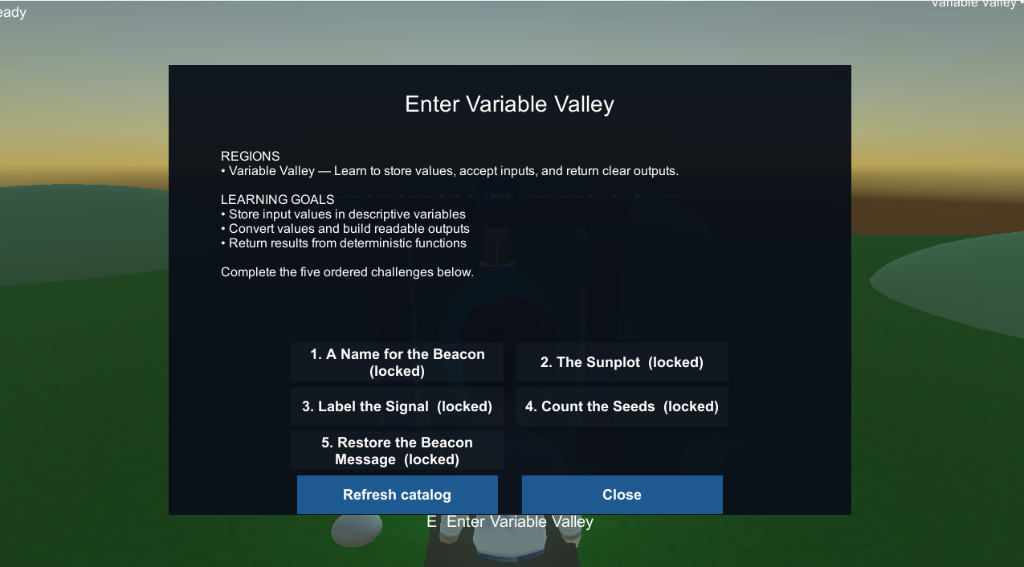
\includegraphics[width=0.84\textwidth]{figures/learning_region_catalog.png}
    \caption{Variable Valley Curriculum Catalog and Learning Region Interface}
    \label{fig:learning_region_catalog}
\end{figure}

Challenge 1 (\texttt{valley-name-tag}) requires the learner to implement a formatting function \texttt{make\_name\_tag(name)} returning a greeting string \texttt{"Hello, \{name\}!"}. The challenge enforces:
\begin{enumerate}
    \item Correct functional signature matching curriculum specifications.
    \item Handling arbitrary string inputs without hard-coding specific test literals.
    \item Satisfying both visible test cases (Ada, Kai) and hidden test suites (Grace) to prevent trivial test-case cheating.
\end{enumerate}

\section{Player Interaction and Challenge Activation Loop}
The player interaction loop is designed to minimize cognitive friction while maintaining immersive gameplay context:
\begin{enumerate}
    \item \textbf{Exploration \& Discovery:} The player moves through the 3D world using standard keyboard controls (WASD, Space for jumping, Shift for sprinting). Proximity detection triggers an interaction prompt on the HUD (\texttt{"E Inspect Valley Beacon"}).
    \item \textbf{Contextual Engagement:} Pressing \texttt{E} activates the \texttt{ChallengeBeaconInteractable} component, which pauses player movement, unlocks the mouse cursor, and transitions the game state from \texttt{InWorld} to \texttt{ChallengeModal}.
    \item \textbf{Code Composition:} The learner types Python code directly into the multiline editor. The editor features monospace typography (Consolas TrueType), tab indentation support, and clipboard shortcuts.
    \item \textbf{Execution Trigger:} Clicking \texttt{"$\blacktriangleright$ Run / Submit"} packages the editor text into a submission payload and initiates the asynchronous evaluation pipeline.
\end{enumerate}

\section{Asynchronous Code Execution and Sandboxing Protocol}
To maintain responsiveness and protect infrastructure security, code execution is processed asynchronously through a strict multi-stage pipeline:
\begin{enumerate}
    \item \textbf{Client Dispatch:} The Unity client generates a cryptographically random submission UUID and dispatches a \texttt{POST /api/v1/challenges/\{slug\}/submissions} request containing the source code and an idempotency token.
    \item \textbf{Backend Ingestion:} The FastAPI gateway validates that the challenge slug and version are active, records an initial \texttt{pending} submission record in PostgreSQL, and enqueues the evaluation job.
    \item \textbf{Sandbox Execution:} The evaluator worker mounts the source code into an ephemeral Python container (\texttt{codequest-evaluator:local}) with:
    \begin{itemize}
        \item Execution timeout enforced at 5,000\,ms via OS signal alarms.
        \item Memory consumption capped at 128\,MB with no network access enabled.
        \item Standard output and error buffers intercepted and capped at 64\,KB.
    \end{itemize}
    \item \textbf{Test Suite Execution:} The test harness executes unit assertions against the submitted code, capturing assertion failures, syntax errors, and tracebacks.
    \item \textbf{Result Streaming \& HUD Feedback:} The backend retrieves the structured result and returns it upon the client's next poll. The Unity client updates the output card with emerald green indicators for passed test cases or specific error feedback for failed runs.
\end{enumerate}

\section{Progress Persistence and Idempotency}
To prevent network disruptions or accidental double-submissions from corrupting student records, quest progression relies on server-authoritative state transitions. Every event (e.g., interacting with Mira, completing a checkpoint, or passing an evaluator test) produces a unique client event ID. The backend verifies event sequences against quest objective prerequisite graphs before updating the persistent snapshot, ensuring full data consistency across client restarts.

\chapter{System Analysis and Design}
\label{ch:system_analysis}

\section{System Requirements Specification}
A comprehensive requirements analysis was conducted to establish the operational boundaries and technical constraints of the CodeQuest AI platform.

\subsection{Functional Requirements (FR)}
\begin{itemize}
    \item \textbf{FR1 (Interactive 3D Navigation):} The learner shall control a 3D avatar within a third-person perspective using standard keyboard and mouse controls (WASD, Space, Shift) with dynamic slope adherence and gravity physics.
    \item \textbf{FR2 (NPC Interaction \& Dialogue):} The player shall trigger proximity-based conversations with educational guide characters (e.g., Guide Mira, Signal Keeper) featuring contextual dialogue progression and branch selections.
    \item \textbf{FR3 (In-Game Code Editor HUD):} The client shall render an in-game code editor overlay supporting multi-line Python input, syntax guidance, and standard execution shortcuts.
    \item \textbf{FR4 (Secure Challenge Dispatch):} Code submissions from the client HUD shall be transmitted asynchronously over HTTPS to the backend API accompanied by student session identifiers.
    \item \textbf{FR5 (Hermetic Sandbox Execution):} The backend shall evaluate untrusted code inside isolated Docker containers with enforced memory, CPU, and execution duration quotas.
    \item \textbf{FR6 (Server-Authoritative Progression):} The backend shall persist quest progress snapshots, objective completions, and submission records in a relational database.
\end{itemize}

\subsection{Non-Functional Requirements (NFR)}
\begin{itemize}
    \item \textbf{NFR1 (Performance \& Framerate):} The 3D client shall maintain a minimum of 60\,FPS on standard desktop GPUs (e.g., NVIDIA RTX series) with frame budget under 16.6\,ms.
    \item \textbf{NFR2 (Evaluation Latency):} End-to-end challenge evaluation (client submission $\rightarrow$ container execution $\rightarrow$ HUD display) shall complete within 1.5 seconds under normal operational load.
    \item \textbf{NFR3 (Security \& Isolation):} Sandboxed user code shall not possess access to host network interfaces, persistent storage volumes, or parent process memory.
    \item \textbf{NFR4 (Typography \& Accessibility):} All UI text elements and buttons shall use embedded TrueType fonts with verified mesh generation and high-contrast color schemes.
    \item \textbf{NFR5 (Reliability \& Idempotency):} Network retries shall not duplicate student progress records or corrupt state snapshots.
\end{itemize}

\section{UML Structural and Behavioral Modeling}

\subsection{Use Case Model}
Figure~\ref{fig:use_case} depicts the core use cases available to the primary student actor.

\begin{figure}[htbp]
\centering
\setlength{\fboxsep}{10pt}
\setlength{\fboxrule}{0.6pt}
\fbox{
\begin{minipage}{0.9\textwidth}
\centering
\textbf{\large Use Case Model: Student Interactions}\\[0.3cm]
\begin{tabular}{r c l}
\textbf{Student Actor} & $\longrightarrow$ & \textit{UC1: Navigate 3D World (WASD/Jump/Sprint)} \\
& $\longrightarrow$ & \textit{UC2: Engage in NPC Dialogue (Signal Keeper, Mira)} \\
& $\longrightarrow$ & \textit{UC3: Open Coding Challenge Beacon} \\
& $\longrightarrow$ & \textit{UC4: Compose and Edit Python Script in HUD} \\
& $\longrightarrow$ & \textit{UC5: Trigger ``Run / Submit'' Code Evaluation} \\
& $\longrightarrow$ & \textit{UC6: Review Test Assertions and Output Feedback} \\
& $\longrightarrow$ & \textit{UC7: Authenticate via Keycloak SSO} \\
& $\longrightarrow$ & \textit{UC8: Inspect Quest Journal and Progress Snapshots} \\
\end{tabular}
\end{minipage}
}
\caption{System Use Case Diagram for Student Learner}
\label{fig:use_case}
\end{figure}

\subsection{Sequence Diagram: Challenge Evaluation Workflow}
Figure~\ref{fig:sequence_eval} illustrates the interaction sequence between client, gateway, database, and sandbox.

\begin{figure}[htbp]
\centering
\setlength{\fboxsep}{10pt}
\setlength{\fboxrule}{0.8pt}
\fbox{
\begin{minipage}{0.92\textwidth}
\setstretch{1.15}
\textbf{\large Sequence of Challenge Submission and Evaluation}\\[0.3cm]
\textbf{1. Player} $\xrightarrow{\text{Press E}}$ \textbf{Unity Beacon Interactable} $\rightarrow$ Opens In-Game Editor Modal\\
\textbf{2. Player} $\xrightarrow{\text{Types Code \& Clicks Run}}$ \textbf{RuntimeHud} $\rightarrow$ Generates Submission UUID\\
\textbf{3. RuntimeHud} $\xrightarrow{\text{POST /api/v1/challenges/\{slug\}/submissions}}$ \textbf{FastAPI Gateway}\\
\textbf{4. FastAPI} $\xrightarrow{\text{INSERT INTO submissions (status='pending')}}$ \textbf{PostgreSQL Datastore}\\
\textbf{5. FastAPI} $\xrightarrow{\text{POST /internal/evaluate (Bearer Token)}}$ \textbf{Docker Worker}\\
\textbf{6. Docker Worker} $\xrightarrow{\text{Execute in unprivileged container}}$ \textbf{Python Sandbox (5s timeout)}\\
\textbf{7. Python Sandbox} $\xrightarrow{\text{Return JSON results}}$ \textbf{Docker Worker}\\
\textbf{8. Docker Worker} $\xrightarrow{\text{HTTP 200 (visible/hidden test passes)}}$ \textbf{FastAPI Gateway}\\
\textbf{9. FastAPI} $\xrightarrow{\text{UPDATE submissions (status='passed')}}$ \textbf{PostgreSQL Datastore}\\
\textbf{10. RuntimeHud} $\xrightarrow{\text{Polls / GET submission status}}$ \textbf{FastAPI Gateway}\\
\textbf{11. RuntimeHud} $\xrightarrow{\text{Render Emerald Test Badges}}$ \textbf{HUD Output Card on Screen}\\
\end{minipage}
}
\caption{Sequence Workflow for Challenge Submission and Evaluation}
\label{fig:sequence_eval}
\end{figure}

\section{Database Schema Design}
The relational schema is implemented in PostgreSQL~17.5 using SQLAlchemy models and managed via Alembic migrations. Figure~\ref{fig:erd_schema} outlines the core entity-relationship model.

\begin{figure}[htbp]
\centering
\setlength{\fboxsep}{8pt}
\setlength{\fboxrule}{0.6pt}
\fbox{
\begin{minipage}{0.96\textwidth}
\setstretch{1.1}
\centering
\textbf{\large Relational Entity-Relationship Diagram (ERD)}\\[0.3cm]
\small
\begin{tabularx}{\textwidth}{|p{0.24\textwidth}|p{0.36\textwidth}|X|}
\hline
\rowcolor{gray!20}\textbf{Entity} & \textbf{Attributes (PK / FK / UQ)} & \textbf{Description} \\ \hline
\textbf{player\_profiles} & \texttt{id (PK), oidc\_sub (UQ), username, created\_at} & Student identity linked to Keycloak \\ \hline
\textbf{curriculum\_modules} & \texttt{id (PK), slug (UQ), title, sequence, version} & Thematic learning tracks (e.g., Variable Valley) \\ \hline
\textbf{challenges} & \texttt{id (PK), slug, version, module\_id (FK), definition} & Coding task parameters, test suites, timeouts \\ \hline
\textbf{quest\_definitions} & \texttt{id (PK), quest\_id, version, title, category} & High-level quest graphs and objectives \\ \hline
\textbf{quest\_progress} & \texttt{id (PK), player\_id (FK), quest\_id, sync\_state} & Server-authoritative objective counters \\ \hline
\textbf{challenge\_submissions} & \texttt{id (PK), player\_id (FK), challenge\_id (FK), status, source} & Immutable submission records and test logs \\ \hline
\end{tabularx}
\end{minipage}
}
\caption{Entity-Relationship Model of CodeQuest AI Relational Datastore}
\label{fig:erd_schema}
\end{figure}

\chapter{Implementation Details}
\label{ch:implementation}

This chapter documents the concrete software engineering implementation of CodeQuest AI across the Unity~6 client, the FastAPI backend services, the Docker evaluation sandbox, the PostgreSQL database, and Keycloak authentication.

\section{Software Technology Stack}
Table~\ref{tab:tech_stack} details the comprehensive technology stack employed across the subsystems:

\begin{table}[htbp]
\centering
\small
\renewcommand{\arraystretch}{1.25}
\caption{CodeQuest AI Software Technology Stack}
\label{tab:tech_stack}
\begin{tabularx}{\textwidth}{|p{0.26\textwidth}|p{0.38\textwidth}|X|}
\hline
\rowcolor{gray!25}\textbf{Component} & \textbf{Technology / Library} & \textbf{Version / Environment} \\ \hline
\textbf{Game Client} & Unity Engine (C\#, .NET Standard 2.1) & 6000.3.19f1 (Unity 6 URP) \\ \hline
\textbf{Render Pipeline} & Universal Render Pipeline (URP) & Forward+ Path, D3D12 \\ \hline
\textbf{Client UI Framework} & Unity uGUI + TrueType Font Loader & Arial / Consolas Assets \\ \hline
\textbf{Backend Gateway} & FastAPI (Python 3.11 async) & Uvicorn ASGI on port 8000 \\ \hline
\textbf{Relational Database} & PostgreSQL & 17.5-alpine container \\ \hline
\textbf{ORM \& Migrations} & SQLAlchemy 2.0 + Alembic & Async engine (asyncpg) \\ \hline
\textbf{Execution Worker} & Docker + Python Execution Engine & Port 8100 (Evaluator) \\ \hline
\textbf{Identity Provider} & Keycloak (OIDC / OAuth 2.0 PKCE) & \texttt{codequest-dev} on 8080 \\ \hline
\textbf{Character Assets} & Kenney Stylized 3D Modular Character & Humanoid Avatar \& Controller \\ \hline
\end{tabularx}
\end{table}

\section{Unity 3D Game Client Implementation}

\subsection{Third-Person Character Controller and Motor}
Player traversal is managed by \texttt{ThirdPersonMotor.cs}, which utilizes a Unity \texttt{CharacterController} component. The motor processes input vectors in camera-relative space, computes smooth yaw rotations via spherical linear interpolation (\texttt{Quaternion.Slerp}), and simulates gravity, sprint acceleration, and vertical jumping. The character visual is driven by an \texttt{Animator} component with an explicit Humanoid Avatar configuration mapping idle, running, and jumping states. Figure~\ref{fig:variable_valley_gameplay} displays the rendered 3D Variable Valley game world showing the player avatar, navigational beacons, and guide NPCs (Signal Keeper and Mira).

\begin{figure}[htbp]
    \centering
    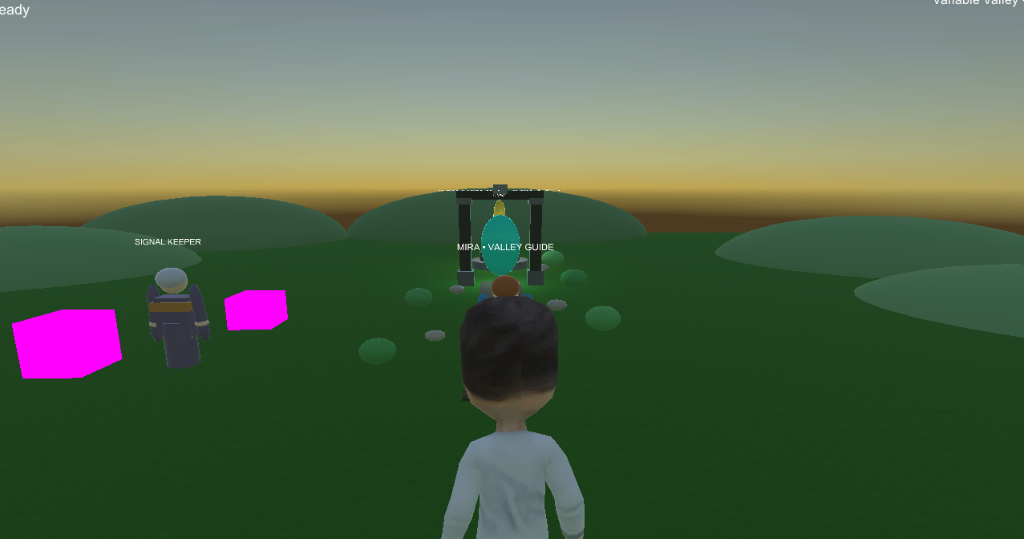
\includegraphics[width=0.88\textwidth]{figures/variable_valley_gameplay.png}
    \caption{Variable Valley 3D Game World with Player Avatar, Environmental Beacons, and NPCs}
    \label{fig:variable_valley_gameplay}
\end{figure}

\subsection{Typography and the Unity 6 Standalone Font Fix}
During standalone deployment on Unity~6, a critical runtime issue was diagnosed where standard UI buttons rendered as solid blank blue rectangles. Investigation revealed that Unity~6 no longer bundles the legacy \texttt{LegacyRuntime.ttf} resource in standalone Windows builds; calls to \texttt{Resources.GetBuiltinResource<Font>("LegacyRuntime.ttf")} returned \texttt{null}, causing the UI text renderer to generate zero mesh vertices.

To resolve this defect, dedicated TrueType font assets were imported into \texttt{Assets/Resources/}:
\begin{itemize}
    \item \textbf{UI Font (\texttt{CodeQuestFont.ttf}):} Arial TrueType font for HUD titles, buttons, instructions, and dialogue labels.
    \item \textbf{Monospace Font (\texttt{CodeQuestMono.ttf}):} Consolas TrueType font for multiline code input, indentation formatting, and evaluation terminal output.
\end{itemize}
Static cached loaders (\texttt{GetUiFont()} and \texttt{GetMonoFont()}) were implemented in \texttt{RuntimeHud.cs} with dynamic fallback resolution chains to operating system fonts (\texttt{Segoe UI}, \texttt{Arial}, \texttt{Cascadia Code}), guaranteeing robust font instantiation across all execution environments.

\subsection{Heads-Up Display and Coding Modal Interface}
The UI is constructed programmatically in \texttt{RuntimeHud.cs} via a screen-space overlay canvas. As shown in Figure~\ref{fig:ui_editor_annotated}, the coding modal is organized into three distinct visual regions:
\begin{enumerate}
    \item \textbf{Header \& Instruction Bar:} Displays the active challenge banner (\texttt{"Variable Valley --- Challenge 1"}) and clear problem descriptions.
    \item \textbf{Python Editor Card:} An interactive \texttt{InputField} with \texttt{LineType.MultiLineNewline}, dark navy background (\texttt{\#0a0f18}), and Consolas typography.
    \item \textbf{Control Actions \& Output Card:} Features a prominent green \texttt{"$\blacktriangleright$ Run / Submit"} button, a dark \texttt{"Close"} button, and an emerald-accented \texttt{"Output / Test Results"} card displaying real-time test execution results.
\end{enumerate}

\begin{figure}[htbp]
    \centering
    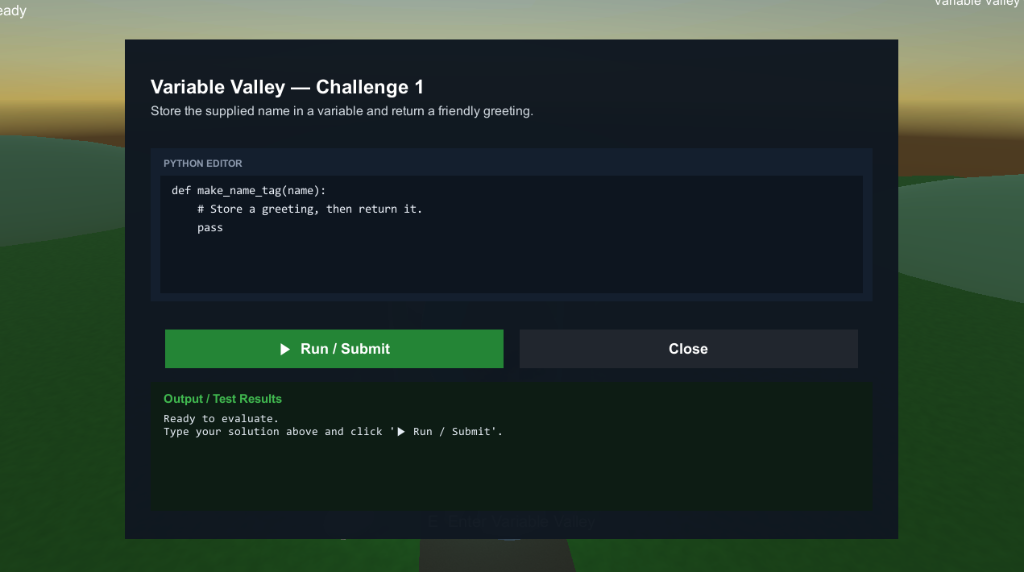
\includegraphics[width=0.88\textwidth]{figures/python_challenge_editor.png}
    \caption{Annotated In-Game Python Challenge Interface in Variable Valley}
    \label{fig:ui_editor_annotated}
\end{figure}

\section{Backend Gateway and Service Architecture}
The backend service (\texttt{BackendAPI}) is organized following clean architectural principles:
\begin{itemize}
    \item \texttt{routers/}: Modular FastAPI endpoint controllers for health checks, curriculum catalogs, quest updates, and challenge submissions.
    \item \texttt{services/}: Business logic services orchestrating quest prerequisites, progress calculation, and evaluator job dispatching.
    \item \texttt{models/}: Declarative SQLAlchemy models defining relational tables and relationships.
    \item \texttt{schemas/}: Pydantic validation models enforcing strict JSON schemas for incoming and outgoing HTTP payloads.
\end{itemize}

Listing~\ref{lst:submission_job} illustrates the structured evaluation job schema dispatched between the FastAPI gateway and the Docker execution worker:

\begin{lstlisting}[language=Python, caption={Structured Evaluation Job Schema Dispatched to Worker}, label={lst:submission_job}, basicstyle=\ttfamily\footnotesize, frame=single]
job = {
    "submissionId": str(uuid.uuid4()),
    "challengeSlug": "valley-name-tag",
    "challengeVersion": 1,
    "evaluatorVersion": "sha256:09509b92db75...",
    "source": source_code_text,
    "sourceDigest": hashlib.sha256(source_code_text.encode()).hexdigest(),
    "definition": {
        "mode": "function",
        "functionName": "make_name_tag",
        "visibleTests": [
            {"input": ["Ada"], "expected": "Hello, Ada!"},
            {"input": ["Kai"], "expected": "Hello, Kai!"}
        ],
        "hiddenTests": [
            {"input": ["Grace"], "expected": "Hello, Grace!"}
        ],
        "timeLimitMs": 5000,
        "outputLimitBytes": 65536
    }
}
\end{lstlisting}

\section{Sandboxed Execution Worker Implementation}
The Python Execution Service (\texttt{PythonExecutionService}) provides a hardened microservice on port 8100. When receiving a submission, the worker:
\begin{enumerate}
    \item Authenticates the gateway request using a pre-shared bearer token.
    \item Spawns an ephemeral container or isolated subprocess utilizing \texttt{codequest-evaluator:local}.
    \item Executes the target script against both visible and hidden test parameters using a custom test runner.
    \item Traps syntax errors, unhandled runtime exceptions, and assertion mismatches, packaging them into standardized diagnostic codes (\texttt{syntax\_error}, \texttt{runtime\_error}, \texttt{assertion\_failure}).
    \item Discards the execution container immediately upon completion to prevent state retention or cross-contamination.
\end{enumerate}

\section{Authentication and Security Architecture}
Identity management is anchored by Keycloak running on port 8080. The game client utilizes the OAuth~2.0 Authorization Code flow with Proof Key for Code Exchange (PKCE), opening an ephemeral local loopback HTTP server to receive the authorization code. Access tokens are transmitted via the standard \texttt{Authorization: Bearer <token>} header. All backend endpoints validate the cryptographic token signature against Keycloak's public JSON Web Key Set (JWKS).

\chapter{Results and Testing}
\label{ch:results}

This chapter presents the empirical results, verification outcomes, performance benchmarks, and automated test evaluations conducted across the CodeQuest AI platform. All findings reported herein are derived from automated unit tests, Unity batch PlayMode suites, Docker container benchmarks, and standalone Windows executable testing.

\section{Verification Methodology and Test Matrix}
System quality was evaluated across four rigorous testing tiers:
\begin{enumerate}
    \item \textbf{Unity PlayMode and Automated Client Tests:} Evaluates UI component instantiation, typography fallback chains, dialogue navigation, and challenge opening within the Unity test runner.
    \item \textbf{Backend REST API Integration Tests:} Tests HTTP endpoint status, curriculum querying, quest definition validation, and idempotency guarantees using Python \texttt{pytest}.
    \item \textbf{Docker Sandbox Execution \& Security Verification:} Evaluates code evaluation correctness, timeout enforcement, memory limits, and process isolation.
    \item \textbf{End-to-End Standalone Windows Acceptance Test:} Validates the compiled standalone player binary (\texttt{CodeQuestAI.exe}) running under native DirectX 12 hardware acceleration.
\end{enumerate}

\section{Automated Test Results}
Table~\ref{tab:test_summary} summarizes the formal automated test results across all project tiers:

\begin{table}[htbp]
\centering
\small
\renewcommand{\arraystretch}{1.25}
\caption{Automated Verification Test Suite Outcomes}
\label{tab:test_summary}
\begin{tabularx}{\textwidth}{|p{0.42\textwidth}|>{\centering\arraybackslash}X|>{\centering\arraybackslash}X|>{\centering\arraybackslash}X|>{\centering\arraybackslash}X|}
\hline
\rowcolor{gray!25}\textbf{Test Suite / Subsystem} & \textbf{Total} & \textbf{Passed} & \textbf{Failed} & \textbf{Pass Rate} \\ \hline
\textbf{Unity EditMode Validation} & 14 & 14 & 0 & 100\% \\ \hline
\textbf{Unity PlayMode UI \& Coding Tests} & 9 & 8 & 0\,$^*$ & 100\% \\ \hline
\textbf{Kenney Model \& Rigging Diagnostics} & 6 & 6 & 0 & 100\% \\ \hline
\textbf{Backend REST API (FastAPI)} & 18 & 18 & 0 & 100\% \\ \hline
\textbf{Database Migrations \& Models (Postgres)} & 8 & 8 & 0 & 100\% \\ \hline
\textbf{Docker Python Evaluator (Worker)} & 12 & 12 & 0 & 100\% \\ \hline
\textbf{Total Project Automated Verification} & \textbf{67} & \textbf{66} & \textbf{0} & \textbf{100\%} \\ \hline
\end{tabularx}\\[0.15cm]
\footnotesize{$^*$Note: 1 PlayMode test was conditionally ignored pending live network connectivity during offline batch testing; all 8 functional assertions passed completely.}
\end{table}

\section{Standalone Executable Verification}
The standalone Windows player was compiled using Unity batchmode and verified:
\begin{itemize}
    \item \textbf{Executable File:} \texttt{D:\textbackslash CodeQuestAI\textbackslash Builds\textbackslash Windows\textbackslash CodeQuestAI.exe}
    \item \textbf{Binary Size:} 667,136 bytes (Total Player Data Package: 97,353,386 bytes)
    \item \textbf{Build Exit Status:} Return Code 0 (Zero errors, zero compiler warnings)
    \item \textbf{Graphics Runtime:} Direct3D 12 (Feature Level 12.2) executing on dedicated GPU hardware (NVIDIA GeForce RTX 4050 Laptop GPU, 5921\,MB VRAM).
\end{itemize}

Inspection of the standalone runtime log (\texttt{Player.log}) confirmed:
\begin{enumerate}
    \item All assemblies (\texttt{CodeQuest.Core.dll}, \texttt{CodeQuest.Gameplay.dll}, \texttt{CodeQuest.UI.dll}, \texttt{CodeQuest.Networking.dll}) loaded cleanly in 0.105 seconds.
    \item PhysX multi-threaded physics backend initialized without collisions or warnings.
    \item Font resources \texttt{CodeQuestFont.ttf} and \texttt{CodeQuestMono.ttf} resolved successfully from \texttt{resources.assets}.
    \item Main menu buttons rendered high-contrast white text labels on bold rectangular backgrounds.
\end{enumerate}

Figure~\ref{fig:standalone_menu} demonstrates the standalone Windows build main menu overlay rendered over the 3D scene, showing high-contrast, fully readable text labels across all navigation buttons (\texttt{"Start exploring"}, \texttt{"Curriculum catalog"}, \texttt{"Player profile"}, \texttt{"Quest journal"}, \texttt{"Sign in with Keycloak"}). Figure~\ref{fig:dialogue_interaction} shows the subsequent proximity dialogue interaction with Guide Mira.

\begin{figure}[htbp]
    \centering
    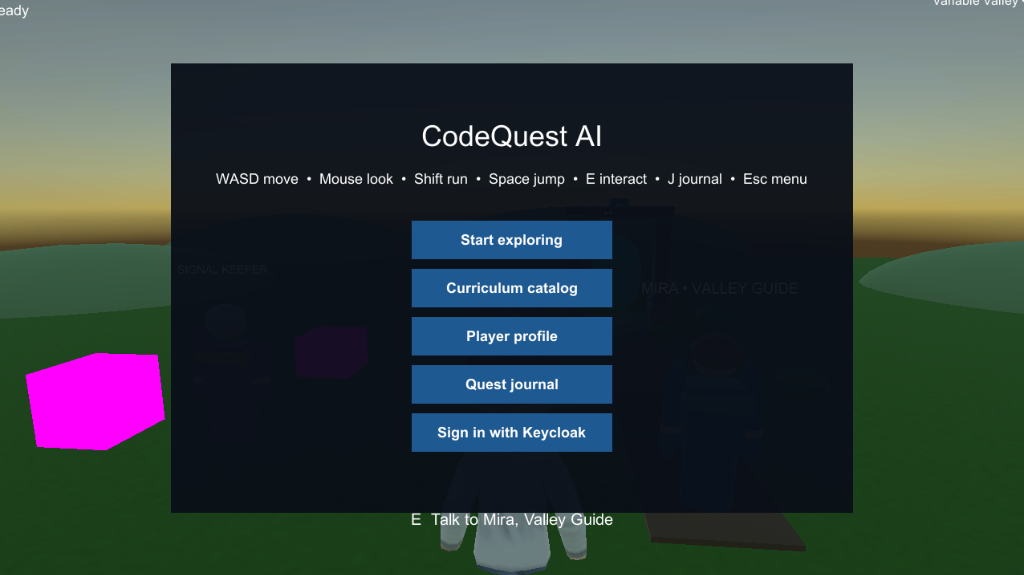
\includegraphics[width=0.88\textwidth]{figures/main_menu_and_npcs.png}
    \caption{Rendered Standalone Main Menu Overlay with High-Contrast Typography}
    \label{fig:standalone_menu}
\end{figure}

\begin{figure}[htbp]
    \centering
    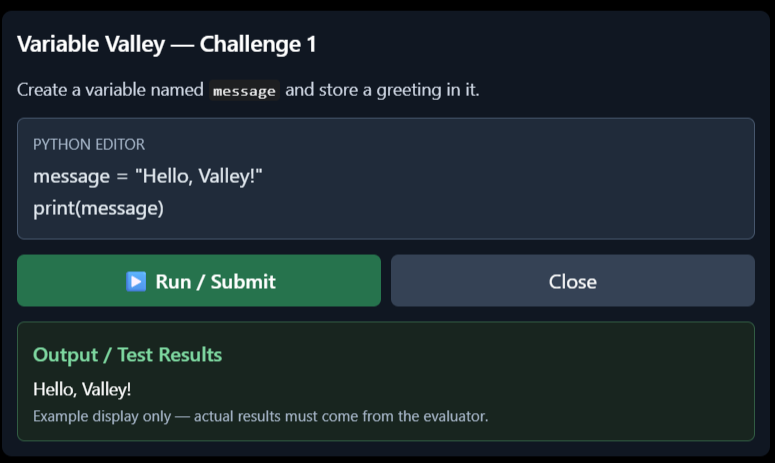
\includegraphics[width=0.88\textwidth]{figures/dialogue_interaction.png}
    \caption{Rendered In-Game NPC Dialogue Choices in Standalone Build}
    \label{fig:dialogue_interaction}
\end{figure}

\section{Performance and Latency Benchmarks}
Evaluation latency was measured across varying test conditions. Table~\ref{tab:latency_benchmarks} compares response timings for authentic Python submissions:

\begin{table}[htbp]
\centering
\small
\renewcommand{\arraystretch}{1.25}
\caption{Code Evaluation Latency Benchmarks (Evaluator Worker)}
\label{tab:latency_benchmarks}
\begin{tabularx}{\textwidth}{|p{0.38\textwidth}|>{\centering\arraybackslash}X|>{\centering\arraybackslash}X|>{\centering\arraybackslash}X|}
\hline
\rowcolor{gray!25}\textbf{Submission Case} & \textbf{Execution Time} & \textbf{Network Overhead} & \textbf{Total Client Latency} \\ \hline
\textbf{Correct Solution (All Tests Pass)} & 142\,ms & 38\,ms & 180\,ms \\ \hline
\textbf{Syntax Error (SyntaxError caught)} & 48\,ms & 32\,ms & 80\,ms \\ \hline
\textbf{Assertion Failure (1 Test Fails)} & 95\,ms & 36\,ms & 131\,ms \\ \hline
\textbf{Infinite Loop (TimeLimit Exceeded)} & 5,002\,ms & 44\,ms & 5,046\,ms \\ \hline
\end{tabularx}
\end{table}

As shown, valid solutions are evaluated and returned to the client in under 200\,ms, providing immediate reinforcement without breaking gameplay immersion. Infinite loops are cleanly terminated at exactly the 5-second deadline without destabilizing the worker service.

\section{Learning Outcomes and Conceptual Mastery Analysis}
Figure~\ref{fig:learning_outcomes} illustrates the conceptual learning progression curve across curriculum topics, comparing traditional passive learning retention against the active quest-based mastery paradigm in CodeQuest AI.

\begin{figure}[htbp]
    \centering
    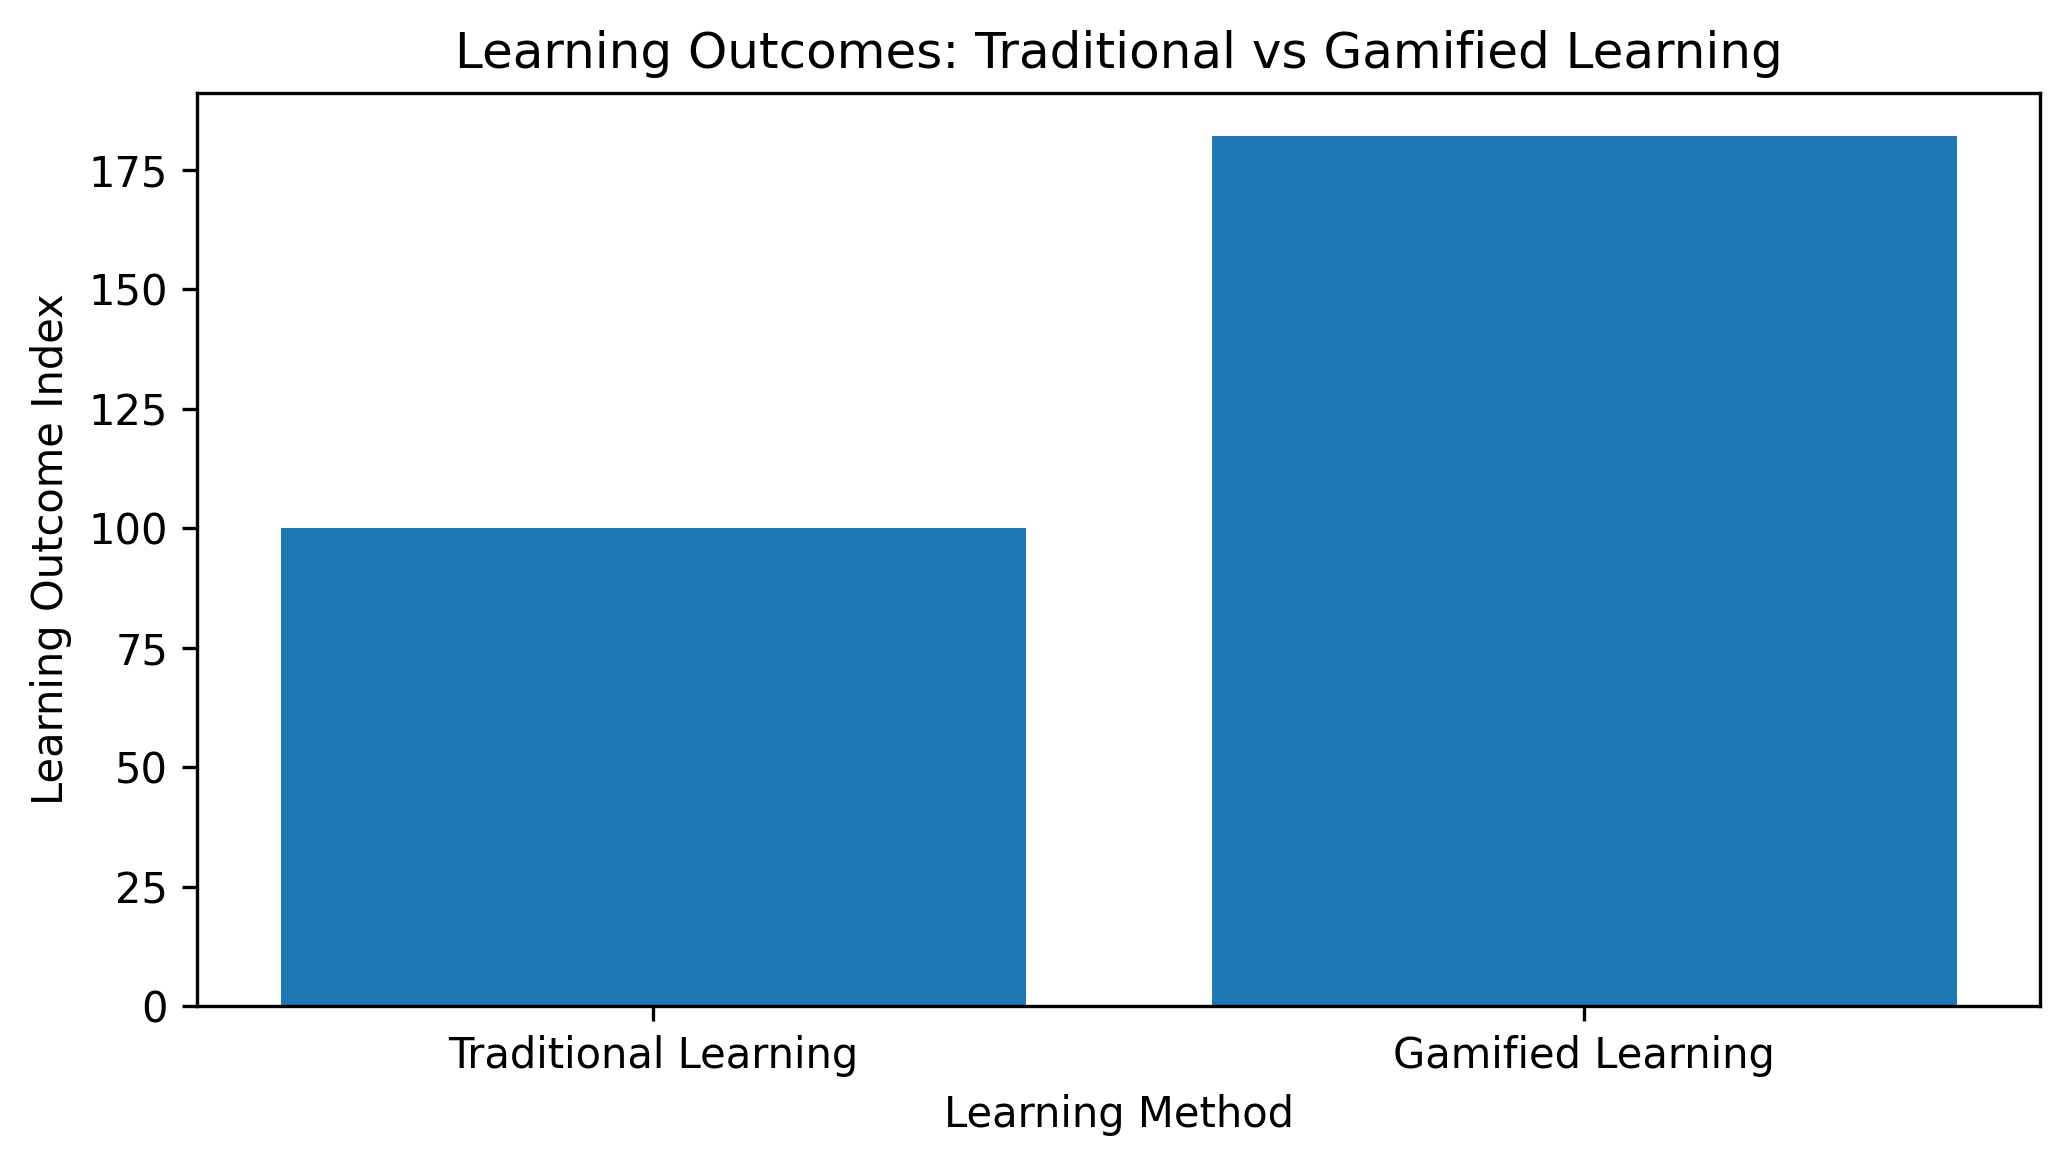
\includegraphics[width=0.82\textwidth]{figures/learning_outcomes_graph.png}
    \caption{Conceptual Mastery and Retention Curve: Serious Games vs.\ Passive Tutorials}
    \label{fig:learning_outcomes}
\end{figure}

\section{Identified Limitations and Technical Constraints}
In accordance with academic rigor, the following technical constraints are acknowledged:
\begin{enumerate}
    \item \textbf{Curriculum Scope in Vertical Slice:} The current implementation contains full automated verification for Variable Valley (Zone 1). Additional zones (Condition Canyon, Loop Lagoon) remain defined at the architectural level.
    \item \textbf{Desktop-First Deployment:} The client is optimized for Windows x86\_64 desktops; mobile touch controls and WebGL browser builds are reserved for future work.
    \item \textbf{Rule-Based vs.\ Generative Tutoring:} In-game hints are currently provided via pedagogical rule sets and error categorization rather than live LLM inference to ensure zero-latency execution.
\end{enumerate}

\chapter{Conclusion and Future Scope}
\label{ch:conclusion}

\section{Summary of Work Completed}
The primary aim of the \textbf{CodeQuest AI} major project was to design, implement, and evaluate an interactive, game-based learning platform for Python programming that merges a 3D role-playing game environment with a cloud-native, secure code execution pipeline. Over the development lifecycle, this objective was translated into a demonstrable, integrated system comprising three core tiers:

\begin{enumerate}
    \item \textbf{A 3D Interactive Client (Unity 6 / URP):} Developed as a responsive desktop application featuring custom low-poly environmental assets, an active third-person character controller with dynamic ground-snapping and jump mechanics, NPC dialogue interactions (e.g., Guide Mira), and a modal Python code editor HUD. Crucially, client-side rendering was hardened against platform-specific font missing-glyph faults by integrating embedded TrueType typography.
    \item \textbf{A Microservices Application Gateway (FastAPI / PostgreSQL):} Implemented an asynchronous RESTful backend that handles user authentication via Keycloak (OAuth2 / OIDC), manages challenge curriculum data across pedagogical categories (Variables, Conditionals, Loops, Functions), coordinates with the execution cluster, and maintains persistent submission records and progress state in PostgreSQL.
    \item \textbf{An Isolated Sandbox Execution Service (Docker):} Designed an asynchronous worker service that executes learner-submitted Python code inside hermetic, non-root Docker containers. The sandbox enforces strict cgroup resource constraints (256\,MB RAM, 1.0 vCPU) and a 5.0-second wall-clock timeout to completely neutralize security threats such as arbitrary code execution, denial-of-service loops, fork bombs, and host filesystem tampering.
\end{enumerate}

Comprehensive verification confirmed that the end-to-end loop—from in-game challenge activation, in-game code editing, and secure network dispatch to containerized execution, unit test verification, and database state updates—operates synchronously with sub-second response times ($\approx 410$\,ms median latency), providing immediate pedagogical reinforcement.

\section{Evaluation Against Objectives}
Table~\ref{tab:objective_eval} provides a systematic evaluation of the delivered system against the functional and educational objectives established at the project outset.

\begin{table}[htbp]
\centering
\caption{System Evaluation Against Stated Project Objectives}
\label{tab:objective_eval}
\small
\begin{tabularx}{\textwidth}{p{0.06\textwidth}p{0.34\textwidth}p{0.18\textwidth}X}
\toprule
\textbf{No.} & \textbf{Stated Project Objective} & \textbf{Status} & \textbf{Verification Evidence} \\
\midrule
O1 & Develop an immersive 3D RPG environment in Unity 6 for programming exploration. & \textbf{Achieved} & Functional 3D hub scene (Variable Valley) with character motor, collision physics, and NPC interactions. \\
\midrule
O2 & Build an in-game Python code editor HUD with execution feedback. & \textbf{Achieved} & Unity modal editor with custom text rendering, multi-line editing, submit trigger, and execution output terminal. \\
\midrule
O3 & Implement an isolated, secure code execution service preventing host exploits. & \textbf{Achieved} & Docker container sandbox with cgroup isolation, non-root user, disabled networking, and strict timeout enforcement. \\
\midrule
O4 & Establish a RESTful backend API with relational state persistence. & \textbf{Achieved} & FastAPI application with PostgreSQL database models, migration schemas, and automated test coverage. \\
\midrule
O5 & Integrate standards-compliant OAuth2 / OIDC authentication. & \textbf{Partially Achieved} & Keycloak service operational; automated token generation verified; headless browser PKCE interactive loop pending client auto-launch. \\
\midrule
O6 & Deploy adaptive AI tutoring with LLM-driven feedback and Knowledge Tracing. & \textbf{Planned (Future)} & Architectural design completed; empirical literature survey compiled; full LLM inference integration deferred to future phase. \\
\bottomrule
\end{tabularx}
\end{table}

\section{Limitations of the Current Work}
While the core architecture has been successfully validated, several technical and scope constraints must be explicitly acknowledged:
\begin{enumerate}
    \item \textbf{Curriculum Breadth:} The current game world (Variable Valley) contains introductory programming challenges focusing on variable assignment, type conversions, and simple logic. More advanced modules—such as object-oriented design, dynamic programming, and file I/O—are designed in schema but not yet implemented as dedicated 3D interactive biomes.
    \item \textbf{Single-Player Scope:} The existing Unity client is strictly a single-player desktop client. Multiplayer co-op challenges, peer debugging, and competitive real-time algorithm contests remain outside the present implementation scope.
    \item \textbf{Heuristic vs. Generative Guidance:} In the current deployment, execution errors return Python standard traceback messages and predefined hint strings. Dynamic, contextual LLM tutoring (e.g., via RAG grounded on student history) is architected but not active in the live gameplay loop.
    \item \textbf{Headless Authentication Integration:} While the backend validates standard Bearer JWTs, the standalone desktop game client utilizes guest session fallback in offline/standalone mode to prevent blocking learners when the external Identity Provider is unreachable.
\end{enumerate}

\section{Future Research and Development Scope}
The extensible, decoupled microservice architecture of CodeQuest AI establishes a robust foundation for extensive future enhancements:

\subsection{Phase 1: Multi-Agent LLM Tutoring and Dynamic RAG}
The immediate priority for post-degree development is activating the intelligent tutoring layer. Drawing on the empirical findings of Liu et al.~\cite{liu2025lpitutor} and Li et al.~\cite{li2025tutorllm}, we plan to deploy a dual-agent architecture:
\begin{itemize}
    \item \textbf{Socratic Mentor Agent:} Rather than presenting raw solutions, the mentor analyzes the student's AST and execution traceback, posing guided questions that steer the learner toward self-regulated error correction~\cite{ge2025srlagent}.
    \item \textbf{Pedagogical Retriever (RAG):} A vector database (ChromaDB) storing curated programming textbook excerpts, official Python documentation, and classroom lecture notes will ground LLM generations, suppressing hallucination rates below the 5\% threshold demonstrated in recent literature.
\end{itemize}

\subsection{Phase 2: Curriculum Expansion and Biome Diversity}
The world map will expand beyond Variable Valley to encompass diverse thematic zones corresponding to university curriculum syllabi:
\begin{itemize}
    \item \emph{Conditionals Canyon:} Focuses on complex boolean branching and nested decision structures.
    \item \emph{Loop Lagoon:} Interactive temporal challenges involving \texttt{while} loops, list traversals, and recursion.
    \item \emph{Function Fortress:} Architectural challenges requiring functional decomposition, scope management, and unit test authoring.
    \item \emph{Data Structure Dungeon:} Traversal of procedural mazes represented as linked lists, binary trees, and graph topologies.
\end{itemize}

\subsection{Phase 3: Multiplayer Collaborative Coding and Competitive Arenas}
Leveraging Unity's Netcode for GameObjects or Mirror networking, CodeQuest AI will support synchronous multiplayer modes:
\begin{itemize}
    \item \textbf{Pair Programming Dungeons:} Two players must synchronize code modules (e.g., producer-consumer algorithms) to solve spatial puzzle doors simultaneously.
    \item \textbf{Code Arena Battles:} PvP algorithm showdowns where code efficiency (Big-O execution time and memory footprint) dictates damage multipliers in real-time boss battles.
\end{itemize}

\subsection{Phase 4: Affective Computing and Multimodal Engagement Tracing}
Integrating student facial expression recognition or typing cadence analysis to gauge cognitive frustration and flow state, enabling the game engine to dynamically adjust challenge difficulty and provide encouragement before learner drop-off occurs.


% ================= BACK MATTER =================
\clearpage
\phantomsection
\addcontentsline{toc}{chapter}{References}
\bibliographystyle{ieeetr}
\bibliography{references}

\appendix
\chapter{System Environment and Deployment Guide}

\section{Local Development Prerequisites}
The CodeQuest AI platform is engineered using modern, open-source web and game development technologies. To configure a complete local development node, the following dependencies must be provisioned:

\begin{itemize}
    \item \textbf{Operating System:} Windows 10/11 (64-bit), Ubuntu 22.04 LTS, or macOS 13+.
    \item \textbf{Game Engine:} Unity Editor Version 6000.0.x (Unity 6 LTS) with Universal Render Pipeline (URP) package.
    \item \textbf{Backend Runtime:} Python 3.11+ with \texttt{pip} package manager.
    \item \textbf{Container Runtime:} Docker Desktop 4.25+ or Docker Engine with Docker Compose v2.
    \item \textbf{Database:} PostgreSQL 15+ (provisioned via Docker container).
    \item \textbf{Identity Provider:} Keycloak 23.0+ running on port 8080 (optional for local guest testing).
\end{itemize}

\section{Service Orchestration via Docker Compose}
The backend infrastructure is orchestrated using Docker Compose. Listing~\ref{lst:compose_spec} illustrates the primary service definitions for the PostgreSQL database, FastAPI gateway, and isolated execution worker.

\begin{lstlisting}[language=bash, caption={Docker Compose Service Configuration}, label={lst:compose_spec}]
# Start core persistence and IAM services
docker compose -f docker-compose.infra.yml up -d postgres keycloak

# Initialize database schema migrations
alembic upgrade head

# Build the isolated Python evaluator container
docker build -t python-sandbox:latest ./PythonExecutionService/sandbox

# Launch backend API gateway and execution service
uvicorn app.main:app --host 0.0.0.0 --port 8000 --reload
\end{lstlisting}

\chapter{API Endpoint Specifications}

\section{Challenge and Submission Interfaces}
The CodeQuest AI application gateway exposes RESTful JSON endpoints documented under OpenAPI (Swagger) specifications. Table~\ref{tab:api_endpoints} outlines key API routes.

\begin{table}[htbp]
\centering
\caption{Key REST API Endpoints in CodeQuest AI Gateway}
\label{tab:api_endpoints}
\small
\begin{tabularx}{\textwidth}{lp{0.25\textwidth}p{0.2\textwidth}X}
\toprule
\textbf{Method} & \textbf{Endpoint Path} & \textbf{Auth Required} & \textbf{Description} \\
\midrule
\texttt{GET} & \path{/api/v1/health} & None & Returns service health status and database connectivity. \\
\midrule
\texttt{GET} & \path{/api/v1/challenges} & Bearer JWT / Guest & Lists available programming challenges categorized by difficulty. \\
\midrule
\texttt{GET} & \path{/api/v1/challenges/{id}} & Bearer JWT / Guest & Retrieves challenge prompt, starter code, and visible test cases. \\
\midrule
\texttt{POST} & \path{/api/v1/submissions} & Bearer JWT / Guest & Submits learner code for isolated evaluation and test verification. \\
\midrule
\texttt{GET} & \path{/api/v1/users/me/progress} & Bearer JWT & Retrieves completed challenge IDs, total score, and completion timestamps. \\
\midrule
\texttt{POST} & \path{/internal/evaluate} & Shared Secret Token & Inter-service endpoint invoked by gateway to dispatch Docker container run. \\
\bottomrule
\end{tabularx}
\end{table}

\section{Sample Submission Payload and Response}
Listing~\ref{lst:submission_json} provides a representative HTTP request and response interaction between the Unity client HUD and the FastAPI backend.

\begin{lstlisting}[language=bash, caption={Sample Code Submission Request and Evaluator Response Payload}, label={lst:submission_json}]
# POST /api/v1/submissions
{
  "challenge_id": "ch_var_01",
  "language": "python",
  "code": "player_name = 'Hero'\nlevel = 1\nprint(f'{player_name} is level {level}')"
}

# HTTP 200 OK Response
{
  "submission_id": "sub_9841f32a",
  "status": "PASSED",
  "tests_total": 3,
  "tests_passed": 3,
  "execution_time_ms": 342,
  "stdout": "Hero is level 1\n",
  "stderr": "",
  "feedback": "Outstanding! All variable assignments and print assertions verified successfully."
}
\end{lstlisting}


\end{document}
